\documentclass{exam}
\usepackage{preamble}
\pagestyle{headandfoot}
\firstpageheader{Physics}{Test on Unit 4: Forces}{}
\CorrectChoiceEmphasis{\color{red}\bfseries}
\SolutionEmphasis{\color{red}}


%\printanswers

\begin{document}
\begin{questions}

\question
Which of the following is the cause of an acceleration or a change in an object's motion?

\question
In the free-body diagram, which is the magnitude of the gravitational force on the balloon?

\begin{figure}[h!]
\centering
\begin{tikzpicture}
\pgfplotsset{compat=1.11}
\def\s{6}
    \begin{axis}[
        width=10cm, height=7cm,
        axis line style={draw=none},
        ticks=none,
        axis lines=middle,
        ymin=-\s, ymax=\s,
        xmin=-\s, xmax=\s,
        clip=false,
    ]
    \fill (0,0) circle (3pt); %node[above=3pt]{\SI{12}{kg}};
    \draw[very thick,black,->] (0,0) -- (0,5.12) node[right] {\SI{5120}{N}};
    \draw[very thick,black,->] (0,0) -- (0.95,0) node[right] {\SI{950}{N}};   
    \draw[very thick,black,->] (0,0) -- (0,-4.05) node[left] {\SI{4050}{N}};
    \draw[very thick,black,->] (0,0) -- (-1.52,0) node[left] {\SI{1520}{N}}; 
    \end{axis}
\end{tikzpicture}
% \caption*{Figure: Free-body diagram of a hot-air balloon. Note: the vertical axis is not to scale with the horizontal one.}
\end{figure}

\question
Which of the following is the tendency of an object to remain at rest or to remain in motion?


\question
Newton said that an apple forcing its weight on a table will experience an upward force on it equal to its weight. This example expemplifies which of Newton's laws?

\question
What is weight?

\question
What is the contact force that acts in the direction opposite to the object's velocity?

% \question
% On Earth, acceleration due to gravity is $g=\SI{9.8}{m/s^2}$. On the Moon, however, acceleration due to gravity is weaker: $g_{\text{moon}} = \SI{1.6}{m/s^2}$. 

\question
A branch weighing \SI{20}{N} falls from the top of a tall tree and experiences \SI{4}{N} of air resistance. What is the magnitude of the net force on the branch?

\question 
The magnitude of the net force required to accelerate a \SI{4.0}{kg} physics book by \SI{2.0}{m/s^2} is \fillin[\SI{8.0}{N}] .

\question
Tweety, the canary who weights \SI{6}{N}, experiences \SI{6}{N} of air resistance as he launches off a branch. What is the net force on Tweety?

\question
A \SI{20}{N} physics book is at rest on a table. What is the magnitude of the force that the table exerts on the book?

\question
When all forces on an object are balanced, which quantity of motion is zero?

\question
What is the weight of a 2.00-kilogram cat?

\question
Two forces act upon a block. If the block's acceleration is \SI{2.0}{m/s^2}, what is mass of the block?

\begin{figure}[h!]
\centering
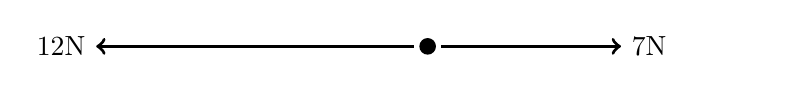
\begin{tikzpicture}
\pgfplotsset{compat=1.11}
\def\s{12}
    \begin{axis}[
        width=10cm, height=2cm,
        axis line style={draw=none},
        ticks=none,
        axis lines=middle,
        ymin=-\s, ymax=\s,
        xmin=-\s, xmax=\s,
        clip=false,
    ]
    \fill (0,0) circle (3pt); %node[above=3pt]{\SI{12}{kg}};
    \draw[very thick,black,->] (0.5,0) -- (7,0) node[right] {\SI{7}{N}};   
    \draw[very thick,black,->] (-0.5,0) -- (-12,0) node[left] {\SI{12}{N}}; 
    \end{axis}
\end{tikzpicture}
\end{figure}

\clearpage
\question
The free-body diagram below shows an object that is accelerating horizontally at \SI{6.0}{m/s^2}. What is the mass of the object?

\begin{figure}[h!]
\centering
\begin{tikzpicture}
\pgfplotsset{compat=1.11}
\def\s{20}
    \begin{axis}[
        width=8cm, height=5cm,
        axis line style={draw=none},
        ticks=none,
        axis lines=middle,
        ymin=-10, ymax=10,
        xmin=-\s, xmax=\s,
        clip=false,
    ]
    \fill (0,0) circle (3pt); %node[above=3pt]{\SI{12}{kg}};
    \draw[very thick,black,->] (1,0) -- (18,0) node[right] {\SI{18}{N}};   
    \draw[very thick,black,->] (-1,0) -- (-6,0) node[left] {\SI{6}{N}}; 
    \draw[very thick,black,->] (0,1) -- (0,10) node[right] {$F_{\text{N}}$}; 
    \draw[very thick,black,->] (0,-1) -- (0,-10) node[right] {$w$};
    \end{axis}
\end{tikzpicture}
\end{figure}

\question
A \SI{45}{kg} object is acted on by a net force of \SI{500}{N}. What is the object's acceleration?

\question
While building the pyramid of Giza, eight people accelerate a 2300-kg block of limestone to \SI{0.800}{m/s^2}, overcoming \SI{3000}{N} of friction. Assume each individual applies the same force. What is magnitude of the force applied by each person? (\textit{Hint}: Draw a free-body diagram.)

\begin{solution}
\vspace{1em}

\textbf{Known}: $a = \SI{0.800}{m/s^2}$, $m = \SI{2300}{kg}$, friction $f = \SI{3000}{N}$. 

\textbf{Unknown}: Individually applied force $F =$ ?

\vspace{1em}

By the vector sum in the free-body diagram,

\begin{equation*}
    F_{\mathrm{net}} = 8F - f\ ,
\end{equation*}

and by Newton's 2nd law (Eq.~4.4),

\begin{equation*}
    F_{\mathrm{net}} = m a = \SI{1840}{N}\ ,
\end{equation*}

implying that

\begin{equation*}
     8F - f = ma\ .
\end{equation*}

Solving for force,

\begin{equation*}
    F = \frac{ma + f}{8} = \SI{605}{N}\ .
\end{equation*}
\end{solution}
\vspace{1em}

\hrule

\begin{EnvUplevel}
\hspace{2cm}
\begin{minipage}{0.6\textwidth}
\textbf{Read the passage below. Then answer the following questions.}\\

Suppose a \SI{10000}{kg} rocket ship blasts off from a launching pad. The upward force is provided by the thrust ($F_{\text{T}}$) from its engines. See the free-body diagram to the right. Assume that the rocket moves only vertically (in a straight line) and that there is no air resistance or friction.
\end{minipage}%
\hspace{-2cm}
\begin{minipage}{0.5\textwidth}
\centering
    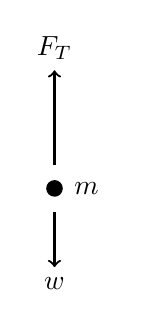
\begin{tikzpicture}
    \fill (0,0) circle[radius=3pt] node[right,inner sep=7pt] {$m$};
    \draw[->, thick] (0,0.3) -- (0,1.5)  node[above] {$F_{\text{T}}$};
    \draw[->, thick] (0,-0.3) -- (0,-1)  node[below] {$w$};
    \end{tikzpicture}
\end{minipage}

\end{EnvUplevel}

\question
Calculate the weight of the rocket.

\question
If the total thrust is \SI{130000}{N}, what is the net force on the rocket during blast-off?
(\textit{Hint}: Use the free-body diagram. In the vertical dimension, we may infer an \textit{up minus down rule})

\question
What is the rocket's vertical acceleration as it blasts off? Assume it moves vertically in one dimension.

\begin{solution}
\vspace{1em}

\textbf{Known}: $m = \SI{1.0e4}{kg}$, thrust $F_{\text{T}} = \SI{1.3e5}{N}$, $g = \SI{9.8}{m/s^2}$

\textbf{Unknown}: $a =$ ?

\begin{center}
    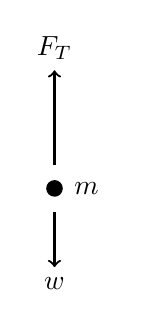
\begin{tikzpicture}
    \fill (0,0) circle[radius=3pt] node[right,inner sep=7pt] {$m$};
    \draw[->, thick] (0,0.3) -- (0,1.5)  node[above] {$F_{\text{T}}$};
    \draw[->, thick] (0,-0.3) -- (0,-1)  node[below] {$w$};
    \end{tikzpicture}
\end{center}

The weight of the rocket is 

\begin{equation*}
    w = m g = \SI{9.8e4}{N}
\end{equation*}

By the vector sum in the free-body diagram, net force is

\begin{equation*}
    F_{\mathrm{net}} = F_{\text{T}} - w = \SI{3.2e4}{N}
\end{equation*}

By Newton's 2nd Law, acceleration is

\begin{equation*}
   a = \frac{F_{\mathrm{net}}}{m} = \SI{3.2}{m/s^2}
\end{equation*}

\end{solution}






\end{questions}
\end{document}